\subsection{Example E10: 3-node recurrent ring / recurrent-network rendering}\label{app:e10-neural}
\paragraph{Purpose.} Demonstrate that a small recurrent network is representable as a motif / closure + wavelet-propagation ledger in which projected non-Markov behavior is a representation adequacy issue and lag/backlog is a clock channel rather than kernel bias.
\paragraph{Depends on.} Collision/export bookkeeping, backlog / forced-dwell bookkeeping, and the CK-mismatch witness on the cited projected stream.
\paragraph{Loss-channel convention.} The primitive loss-facing channel is reported here as $R_{\mathrm{loss}}$ [trit/bip], with the same values as the loss channel on the cited row.
\paragraph{Cited row(s).}
{\footnotesize
\begin{center}
\begin{tabular}{@{}llllllll@{}}
\toprule
Row & topology & $R_{\mathrm{loss}}$ [trit/bip] & $B^*$ & $\widehat\Lambda$ & $R_{\mathrm{loss}}^{(\mathrm{biz})}$ & CK mismatch & $\mathcal R_{\mathrm{cut}}$ \\
\midrule
E10.N1 & 3-node ring & $0.4887777778$ & $2$ & $3$ & $0.0888534592$ & $0.0638525823$ & $0$ \\
\bottomrule
\end{tabular}
\end{center}}
\paragraph{Backlog / dwell slice.}
{\footnotesize
\begin{center}
\begin{tabular}{@{}lllllll@{}}
\toprule
$t$ & node & $\tau_\alpha$ & $\tau_\omega$ & delay [bip] & hidden mode & backlog \\
\midrule
0 & A & $+1$ & $0$ & $3$ & $0$ & $1$ \\
1 & B & $+1$ & $0$ & $2$ & $0$ & $2$ \\
2 & -- & $0$ & $0$ & $0$ & $0$ & $2$ \\
3 & -- & $0$ & $-2$ & $0$ & $0$ & $0$ \\
4 & C & $-1$ & $0$ & $2$ & $0$ & $1$ \\
\bottomrule
\end{tabular}
\end{center}}
\paragraph{Diagrammatic rendering.} The same cited row may be rendered as a three-node recurrent network with node activations and signed transport on the ring $A\to B\to C\to A$. This rendering follows the cited row.
\begin{center}
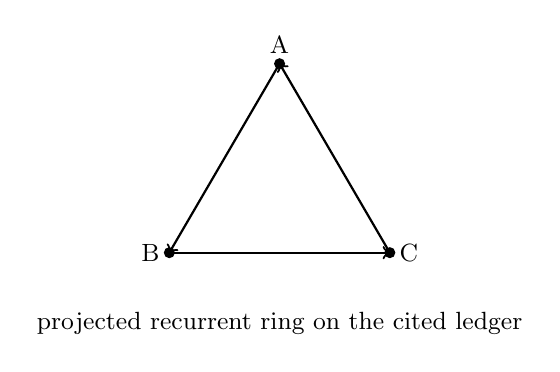
\begin{tikzpicture}[x=1cm,y=1cm, every node/.style={font=\small}]
  \coordinate (A) at (0,1.6);
  \coordinate (B) at (-1.4,-0.8);
  \coordinate (C) at (1.4,-0.8);
  \draw[thick,->] (A) -- (B);
  \draw[thick,->] (B) -- (C);
  \draw[thick,->] (C) -- (A);
  \fill (A) circle (2pt) node[above] {A};
  \fill (B) circle (2pt) node[left] {B};
  \fill (C) circle (2pt) node[right] {C};
  \node at (0,-1.7) {projected recurrent ring on the cited ledger};
\end{tikzpicture}
\end{center}
\paragraph{Audit cues.} Use the CK residual $\|P^{(2)}-P^{(1)}P^{(1)}\|_F$, backlog/dwell columns, and cut residual to distinguish hidden-state projection effects from kernel bias.
